\chapter{Training Report}

\label{chapter:TrainingReport}

% ----------------

\begin{figure*}
	\centering
	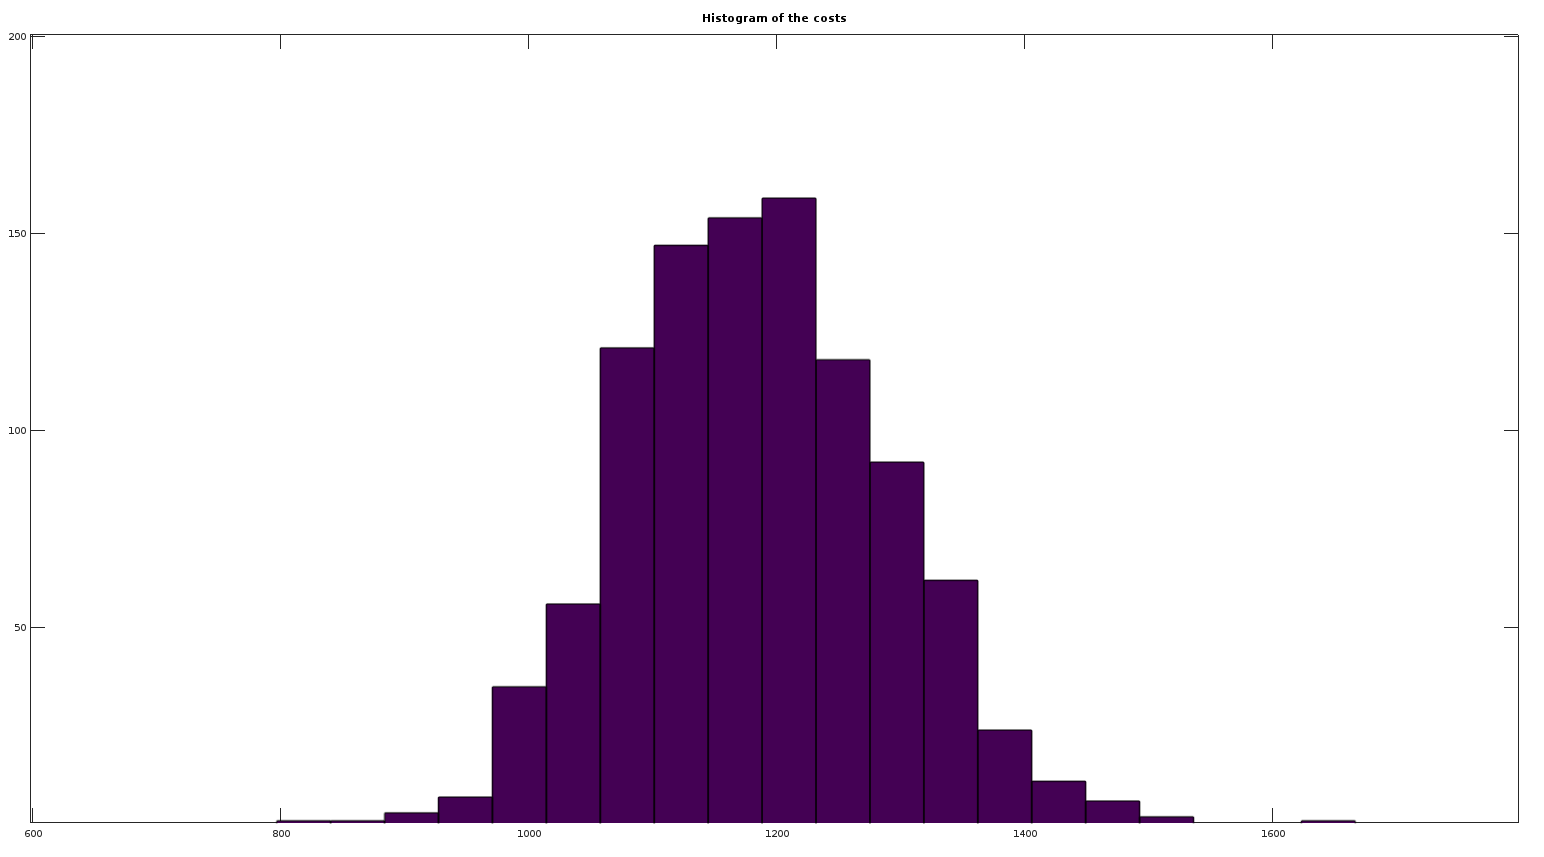
\includegraphics[width=\textwidth]{img/lsh_best_of_1000.png}
	\caption{Histogram of the real cost of 1000 iterations of LSH}
	\label{fig:lsh_best_of_1000}
\end{figure*}

\lstset{
	language={},
	breaklines=true,
  postbreak=\mbox{\textcolor{red}{$\hookrightarrow$}\space}
}
\begin{lstlisting}
initial_cont_cost =  3000.3
initial_real_cost =  1006.0
optimal_real_cost =  27.985
optimal_cont_cost =  0.020816

------ Real cost statistics: ------
Min: 27.9854
Max: 64.9679
Median: 55.3994
Mean: 49.4509
Standard deviation: 19.1954

------ Analysis ------
Middle activation: 1721
Number of training samples: 61075
Number of similar triplets: 1050
Number of dissimilar triplets: 60025
Ratio of similar triplets: 0.017192
Number of true positives: 1031
Number of false positives: 278
Number of false negatives: 19
Number of false negatives: 59747
Ratio of preserved similar triplets: 0.981905
Ratio of preserved dissimilar triplets: 0.995369
Precision: 0.787624
Recall: 0.981905
F1-measure: 0.874099
\end{lstlisting}
